% src/main.tex
\documentclass[xcolor={dvipsnames}]{beamer}

% src/style/preamble.tex

% ==========================================
% 1. METADATA & MACROS (Must be first for the footline)
% ==========================================
\newcommand{\MyTitle}{Efficient Data Structures for \\ \small RDD-based Apriori on Spark}
\newcommand{\MyShortTitle}{Apriori on Spark}
\newcommand{\MyAuthor}{Luis Alberto Vásquez Vargas}
\newcommand{\MyShortAuthor}{Luis Vásquez}
\newcommand{\MyInstitute}{IC -- UNICAMP} 
\newcommand{\MyEmail}{l322989@dac.unicamp.br}
\newcommand{\MyDate}{April 7, 2026} 

\title[\MyShortTitle]{\MyTitle}
\author[\MyShortAuthor]{\MyAuthor}
\institute{\MyInstitute}
\date{\MyDate}

% ==========================================
% 2. PACKAGES
% ==========================================
\usepackage[english]{babel}
\usepackage[utf8]{inputenc}
\usepackage[T1]{fontenc}
\usepackage{beramono}    % Professional code font
\usepackage{amsmath, amsfonts, amssymb}
\usepackage{chemfig}
\usepackage[version=3]{mhchem}
\usepackage{tikz}
\usepackage[table, dvipsnames]{xcolor}

% --- IMAGE PATH ---
% Note: Since you use TEXINPUTS=./src//: in your latexmk command, 
% LaTeX will look recursively for the "img" folder.
\graphicspath{ {img/} }

% ==========================================
% 3. COLORS & THEME SETUP
% ==========================================
\definecolor{PrimaryColor}{HTML}{141B41}
\definecolor{SecondaryColor}{HTML}{306BAC}
\definecolor{AccentColor}{HTML}{6F9CEB}
\definecolor{LightAccent}{HTML}{98B9F2}
\definecolor{AlertColor}{HTML}{918EF4}

\hypersetup{
    colorlinks=true,
    citecolor=SecondaryColor,
    linkcolor=SecondaryColor,
    urlcolor=AccentColor
}

\mode<presentation>
{
  \usetheme{Madrid}
  \usecolortheme{default}
  \usefonttheme{serif}
  \setbeamertemplate{navigation symbols}{}
  
  % --- CUSTOM FOOTLINE ---
  \setbeamertemplate{footline}{
    \leavevmode%
    \hbox{%
    \begin{beamercolorbox}[wd=.4\paperwidth,ht=2.25ex,dp=1ex,center]{author in head/foot}%
      \usebeamerfont{author in head/foot}\MyShortAuthor~~\textbar~~\MyInstitute
    \end{beamercolorbox}%
    \begin{beamercolorbox}[wd=.3\paperwidth,ht=2.25ex,dp=1ex,center]{title in head/foot}%
      \usebeamerfont{title in head/foot}\MyShortTitle
    \end{beamercolorbox}%
    \begin{beamercolorbox}[wd=.3\paperwidth,ht=2.25ex,dp=1ex,right]{date in head/foot}%
      \usebeamerfont{date in head/foot}\insertshortdate{}\hspace*{2em}
      \insertframenumber{} / \inserttotalframenumber\hspace*{2ex} 
    \end{beamercolorbox}}%
    \vskip0pt%
  }

  % --- BEAMER COLORS ---
  \setbeamercolor{structure}{fg=SecondaryColor}
  \setbeamercolor{palette primary}{bg=PrimaryColor, fg=white}
  \setbeamercolor{palette secondary}{bg=SecondaryColor, fg=white}
  \setbeamercolor{palette tertiary}{bg=AccentColor, fg=white}
  \setbeamercolor{titlelike}{parent=palette primary}
  
  \setbeamercolor{author in head/foot}{fg=white, bg=PrimaryColor}
  \setbeamercolor{title in head/foot}{fg=white, bg=SecondaryColor}
  \setbeamercolor{date in head/foot}{fg=white, bg=AccentColor}
  
  \setbeamercolor{block title}{bg=SecondaryColor, fg=white}
  \setbeamercolor{block body}{bg=LightAccent!20, fg=PrimaryColor}
  \setbeamercolor{alerted text}{fg=AlertColor}
  
  % --- BEAMER FONTS ---
  \setbeamerfont{author in head/foot}{size=\tiny}
  \setbeamerfont{title in head/foot}{size=\tiny}
  \setbeamerfont{date in head/foot}{size=\tiny}

  \setbeamertemplate{sections/subsections in toc}[ball]
  \setbeamercolor{section number projected}{bg=PrimaryColor, fg=white}
  \setbeamercolor{subsection number projected}{bg=SecondaryColor, fg=white}
}


\begin{document}

% sections/00_title.tex

\begin{frame}[plain]
  \vfill
  \centering
  \begin{beamercolorbox}[sep=12pt,center,rounded=true]{palette primary}
      \usebeamerfont{title}\inserttitle
  \end{beamercolorbox}
  
  \vspace{0.6cm}
  \textbf{\insertauthor} \\
  \textit{\small \MyInstitute}
  
  \vfill
  \begin{beamercolorbox}[sep=8pt,center,rounded=true]{block body}
      \textbf{MO809 -- Topics in Distributed Computing} \\
      \vspace{0.1cm}
      \small \textbf{Instructor:} Prof. Luiz Fernando Bittencourt
  \end{beamercolorbox}
  
  \vfill
  \scriptsize
  \texttt{\MyEmail} \\
  \MyDate
\end{frame}


\begin{frame}{Outline}
  \tableofcontents[hideallsubsections] % This will now show 1, 2, 3...
\end{frame}

% sections/01_base_study.tex

\section{The Base Study}
\begin{frame}{The Base Study}
    \vspace{-0.2cm} 
    \begin{alertblock}{Original Research Paper}
        \centering
        \textbf{A Data Structure Perspective to the RDD-based Apriori Algorithm on Spark}
    \end{alertblock}
    
    \vspace{0.1cm}
    
    \begin{itemize}
        \setlength{\itemsep}{2pt}
        \item \textbf{Source:} \textit{International Journal of Information Technology} (Springer), 2019.
        \item \textbf{Keywords:} \textit{Parallel Algorithms, Big Data, Apriori, Spark, RDD.}
        \item \textbf{Authors \& Affiliations:} \hspace{0.1cm} 
                
\begin{tikzpicture}[scale=0.08, baseline=-0.5ex]
                    \draw[fill=orange] (0,1.2) rectangle (3,1.8);
                    \draw[fill=white] (0,0.6) rectangle (3,1.2);
                    \draw[fill=green!70!black] (0,0) rectangle (3,0.6);
                    \draw[blue!80!black] (1.5,0.9) circle (0.22);
                    \draw[very thin] (0,0) rectangle (3,1.8);
                \end{tikzpicture}
        \begin{itemize}
            \setlength{\itemsep}{0pt}
            \scriptsize
            \item \textbf{Pankaj Singh \& P. K. Mishra:} Dept. of Computer Science, BHU.
            \item \textbf{Sudhakar Singh:} Dept. of Electronics \& Comm., Univ. of Allahabad.
            \item \textbf{Rakhi Garg:} Mahila Maha Vidyalaya, BHU, Varanasi.
        \end{itemize}
    \end{itemize}

    \vspace{0.2cm}

    % --- AUTHOR PHOTOS ROW ---
    \centering
    \begin{columns}[onlytextwidth, c]
        \begin{column}{0.22\textwidth}
            \centering
            
\includegraphics[width=1.1cm, height=1.3cm, keepaspectratio]{pankaj_singh.png} \\
            {\fontsize{4pt}{5pt}\selectfont Pankaj Singh}
        \end{column}
        \begin{column}{0.22\textwidth}
            \centering
            
\includegraphics[width=1.1cm, height=1.3cm, keepaspectratio]{sudhakar_singh.png} \\
            {\fontsize{4pt}{5pt}\selectfont Sudhakar Singh}
        \end{column}
        \begin{column}{0.22\textwidth}
            \centering
            
\includegraphics[width=1.1cm, height=1.3cm, keepaspectratio]{pk_mishra.png} \\
            {\fontsize{4pt}{5pt}\selectfont P. K. Mishra}
        \end{column}
        \begin{column}{0.22\textwidth}
            \centering
            
\includegraphics[width=1.1cm, height=1.3cm, keepaspectratio]{rakhi_garg.jpg} \\
            {\fontsize{4pt}{5pt}\selectfont Rakhi Garg}
        \end{column}
    \end{columns}

    \vfill 
    \footnotesize
    \centering
    \textbf{Focus:} Comparative efficiency of \textbf{Hash Tree}, \textbf{Trie}, and \textbf{Hash Table Trie} in distributed Spark environments.
\end{frame}

% sections/02_intro.tex

\section{Introduction \& Motivation}

% --- SLIDE 1: The Pipeline (Full Width Visual) ---
\begin{frame}{The Market Basket Problem: From Paper to Patterns}
    \centering
    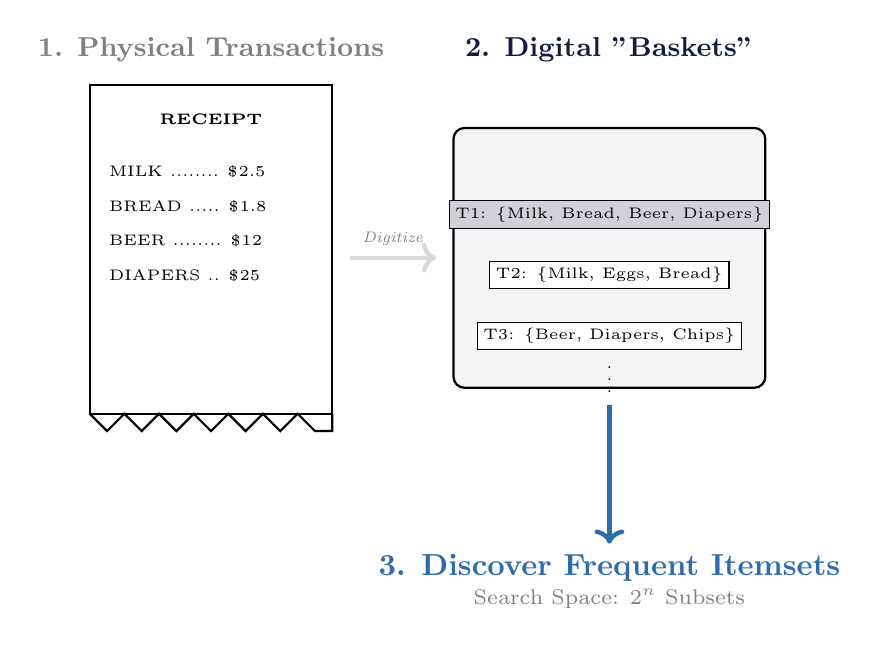
\begin{tikzpicture}[scale=1.1, every node/.style={transform shape}]
        % --- STAGE 1: Physical Data ---
        \node[font=\bfseries\small, gray] at (1.4, 6.2) {1. Physical Transactions};
        \draw[thick, fill=white] (0,2) rectangle (2.8,5.8);
        \draw[thick] (0,2) -- (0.2,1.8) -- (0.4,2) -- (0.6,1.8) -- (0.8,2) -- (1.0,1.8) -- (1.2,2) -- (1.4,1.8) -- (1.6,2) -- (1.8,1.8) -- (2.0,2) -- (2.2,1.8) -- (2.4,2) -- (2.6,1.8) -- (2.8,1.8) -- (2.8,2);
        
        \node at (1.4, 5.4) {\textbf{\tiny RECEIPT}};
        \node[anchor=west] at (0.1, 4.8) {\tiny MILK ........ \$2.5};
        \node[anchor=west] at (0.1, 4.4) {\tiny BREAD ..... \$1.8};
        \node[anchor=west] at (0.1, 4.0) {\tiny BEER ........ \$12};
        \node[anchor=west] at (0.1, 3.6) {\tiny DIAPERS .. \$25};
        
        % --- Transition Arrow 1 ---
        \draw[->, ultra thick, gray!30] (3.0, 3.8) -- (4.0, 3.8) node[midway, above, font=\tiny\itshape, text=gray] {Digitize};

        % --- STAGE 2: Digital Representation ---
        \node[font=\bfseries\small, PrimaryColor] at (6.0, 6.2) {2. Digital "Baskets"};
        \draw[thick, rounded corners, fill=PrimaryColor!5] (4.2, 2.3) rectangle (7.8, 5.3);
        
        \node[draw, fill=PrimaryColor!20, inner sep=2pt] at (6.0, 4.3) {\tiny T1: \{Milk, Bread, Beer, Diapers\}};
        \node[draw, fill=white, inner sep=2pt] at (6.0, 3.6) {\tiny T2: \{Milk, Eggs, Bread\}};
        \node[draw, fill=white, inner sep=2pt] at (6.0, 2.9) {\tiny T3: \{Beer, Diapers, Chips\}};
        \node at (6.0, 2.5) {\tiny $\vdots$};

        % --- Transition Arrow 2 ---
        \draw[->, ultra thick, SecondaryColor] (6.0, 2.1) -- (6.0, 0.5);
        
        % --- STAGE 3: Knowledge Discovery ---
        \node[below, SecondaryColor, font=\bfseries] at (6.0, 0.5) {3. Discover Frequent Itemsets};
        \node[below, font=\scriptsize, text=gray] at (6.0, 0.1) {Search Space: $2^n$ Subsets};
    \end{tikzpicture}
\end{frame}

% --- SLIDE 2: Simple Examples & Goal ---
\begin{frame}{Mining Actionable Patterns}
    \textbf{Examples of Association Rules:}
    \vspace{0.3cm}
    \begin{itemize}
        \item \small $\{Milk, Bread\} \implies \{Eggs\}$
        \item \small $\{Beer\} \implies \{Diapers\}$
        \item \small $\{Wine\} \implies \{Cheese\}$
        \item \small $\{Laptop\} \implies \{Mouse, Keyboard\}$
    \end{itemize}

    \vfill

    \begin{alertblock}{The Data Mining Goal}
        \centering \textbf{Find all subsets of items (itemsets) that appear in at least $s$ transactions within a massive dataset.}
    \end{alertblock}
    
    \vspace{0.4cm}
    \begin{itemize}
        \item \small \textbf{Applications:} Cross-selling, inventory management, and store layout optimization.
    \end{itemize}
\end{frame}

% --- SLIDE 3: The Technical Challenge ---
\begin{frame}{The Technical Challenge: Complexity}
    \begin{columns}[T, onlytextwidth]
        \begin{column}{0.60\textwidth}
            \centering
            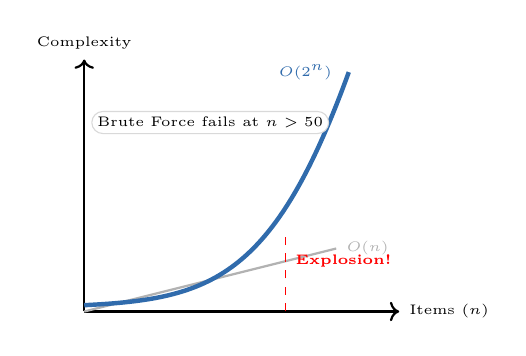
\begin{tikzpicture}[scale=0.8]
                % Axes
                \draw[->, thick] (0,0) -- (5,0) node[right, font=\tiny] {Items ($n$)};
                \draw[->, thick] (0,0) -- (0,4) node[above, font=\tiny] {Complexity};
                
                % Linear Curve O(n)
                \draw[thick, gray!60] (0,0) -- (4,1) node[right, font=\tiny] {$O(n)$};
                
                % Exponential Curve O(2^n)
                \draw[ultra thick, SecondaryColor] (0,0.1) .. controls (2,0.2) and (3,0.5) .. (4.2,3.8) 
                    node[left, font=\tiny, xshift=-2pt] {$O(2^n)$};
                
                % Explosion Marker
                \draw[dashed, red] (3.2,0) -- (3.2,1.2);
                \node[red, font=\tiny\bfseries, anchor=west] at (3.2, 0.8) {Explosion!};
                
                % Annotations
                \node[fill=white, draw=gray!30, rounded corners, font=\tiny, inner sep=2pt] at (2,3) {Brute Force fails at $n > 50$};
            \end{tikzpicture}
            
            \vspace{0.4cm}
            \scriptsize
            $n=100 \implies 2^{100}$ subsets. \\
            $\approx 3,000\times$ Age of Universe by Brute Force.
        \end{column}

        \begin{column}{0.38\textwidth}
            \centering
            \begin{minipage}{\textwidth}
                \centering
                \textbf{Power Set for $n=4$} \\
                \vspace{0.1cm}
                \renewcommand{\arraystretch}{1.1}
                \scriptsize
                \begin{tabular}{l l}
                    \hline
                    \textbf{Size} & \textbf{Subsets} \\ \hline
                    $k=0$ & $\emptyset$ \\
                    $k=1$ & $\{a\}, \{b\}, \{c\}, \{d\}$ \\
                    $k=2$ & $\{ab\}, \{ac\}, \{ad\}, \dots$ \\
                    $k=3$ & $\{abc\}, \{abd\}, \dots$ \\ 
                    $k=4$ & $\{abcd\}$ \\ \hline
                \end{tabular}
                \vspace{0.2cm}
                \small \textbf{Total: 16 Combinations} \\
                \scriptsize \textit{Adding 1 item doubles the work!}
            \end{minipage}
        \end{column}
    \end{columns}

    \vfill 
    \begin{alertblock}{}
        \centering \footnotesize
        \textbf{The Bottleneck:} Exponential $O(2^n)$ combinatorial complexity makes massive-scale association rule mining compute-bound.
    \end{alertblock}
\end{frame}

% --- SLIDE 4: The Infrastructure Solution ---
\begin{frame}{The Infrastructure Solution}
    \begin{columns}[c, onlytextwidth]
        \begin{column}{0.5\textwidth}
            \centering
            \begin{tikzpicture}
                \node[anchor=south west,inner sep=0] (image) at (0,0) {
\includegraphics[width=\textwidth]{img/ferrari.jpg}};
                \node[align=center, fill=PrimaryColor, text=white, font=\bfseries, rounded corners=2pt, inner sep=4pt] 
                    at (2.5, 4.0) {Apache Spark RDDs};
            \end{tikzpicture}
        \end{column}

        \begin{column}{0.45\textwidth}
            \begin{itemize}
                \item \textbf{Hardware Evolution:} 
                \begin{itemize}
                    \item We use \textbf{Apache Spark RDDs}: the distributed ``Ferrari'' of in-memory computing.
                \end{itemize}
                \vspace{0.3cm}
                \item \textbf{The Bottleneck:} 
                \begin{itemize}
                    \item Legacy structures (Hash Trees) act like a \textbf{traffic jam} in a high-speed engine.
                \end{itemize}
            \end{itemize}
        \end{column}
    \end{columns}

    \vfill
    \begin{alertblock}{The Core Thesis}
        Infrastructure alone cannot solve $O(2^n)$. To exploit Spark's speed, we must replace ``Disk-era'' structures with memory-optimized \textbf{Tries}.
    \end{alertblock}
\end{frame}

% sections/03_the_problem.tex

\section{The FIM Problem}

\begin{frame}{Origins and Definition}
    \begin{itemize}
        \item \textbf{Market Basket Analysis:} The historical root of FIM. 
        \item \textbf{The Item Base:} Let $\mathcal{B} = \{i_1, \dots, i_n\}$ be the set of all possible items.
        \item \textbf{Itemsets:} Any subset $I \subseteq \mathcal{B}$.
        \item \textbf{Transactions:} A database $\mathcal{T} = (t_1, \dots, t_m)$ where each transaction $t_k$ is an itemset.
    \end{itemize}

    \vfill

    \begin{alertblock}{Frequent Itemset Mining (FIM)}
        The task of discovering all itemsets $I$ that appear in the database $\mathcal{T}$ with a frequency (support) greater than or equal to a threshold $s_{min}$:
        \[ s_{\mathcal{T}}(I) = |\{k \in \{1, \dots, m\} \mid I \subseteq t_k\}| \geq s_{min} \]
    \end{alertblock}
\end{frame}

\begin{frame}{Illustrative Example}
    \begin{columns}
        \begin{column}{0.45\textwidth}
            \textbf{Transaction Database ($\mathcal{T}$)}
            \footnotesize
            \begin{itemize}
                \item[0:] $\{a, d, e\}$ \quad 5: $\{a, c, d\}$
                \item[1:] $\{b, c, d\}$ \quad 6: $\{b, c\}$
                \item[2:] $\{a, c, e\}$ \quad 7: $\{a, c, d, e\}$
                \item[3:] $\{a, c, d, e\}$ \ 8: $\{b, c, e\}$
                \item[4:] $\{a, e\}$ \quad 9: $\{a, d, e\}$
            \end{itemize}
        \end{column}
        
        \begin{column}{0.55\textwidth}
            \textbf{Frequent Itemsets ($s_{min} = 3$)}
            \scriptsize
            \begin{table}
                \centering
                \begin{tabular}{|l|l|l|}
                \hline
                \textbf{1 item} & \textbf{2 items} & \textbf{3 items} \\ \hline
                $\{a\}: 7$ & $\{a, c\}: 4$ & $\{a, c, d\}: 3$ \\
                $\{b\}: 3$ & $\{a, d\}: 5$ & $\{a, c, e\}: 3$ \\
                $\{c\}: 7$ & $\{a, e\}: 6$ & $\{a, d, e\}: 4$ \\
                $\{d\}: 6$ & $\{b, c\}: 3$ & \\
                $\{e\}: 7$ & $\{c, d\}: 4$ & \\
                           & $\{c, e\}: 4$ & \\
                           & $\{d, e\}: 4$ & \\ \hline
                \end{tabular}
            \end{table}
        \end{column}
    \end{columns}

    \vfill

    \begin{alertblock}{The Search Space Challenge}
        Even for a base of only 5 items, there are $2^5 = 32$ possible itemsets. As $|\mathcal{B}|$ grows, the number of candidates becomes the primary computational bottleneck.
    \end{alertblock}
\end{frame}

% sections/04_infrastructure.tex

\section{Infrastructure Evolution}

% --- Slide 1: The Pre-Big Data Crisis ---
\begin{frame}{The Context: Why now and not before?}
    Before 2004, "Big Data" was handled by massive, expensive vertical mainframes. 

    \begin{columns}
        \begin{column}{0.65\textwidth}
            \begin{itemize}
                \item \textbf{The "Single Giant" (Vertical):} 
                    Hitting the physical and financial ceiling of a single machine.
                \item \textbf{The "Army of Ants" (Horizontal):} 
                    Linking 1,000 "commodity" PCs to act as one.
            \end{itemize}
            \vfill
            \begin{alertblock}{Economic Necessity}
                In the 90s, RAM was \textbf{>\$50/MB}. We switched because scaling vertically became \textbf{bankrupting}.
            \end{alertblock}
        \end{column}
        
        \begin{column}{0.35\textwidth}
            \centering
            % --- TikZ Floppy (Scaled 1.6x) ---
            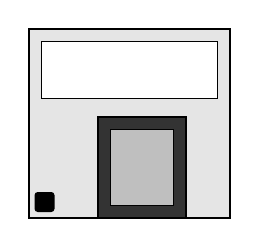
\begin{tikzpicture}[scale=0.8] 
                \draw[thick, fill=gray!20] (0,0) rectangle (3.2, 3.0);
                \draw[fill=white] (0.2, 1.9) rectangle (3.0, 2.8);
                \draw[thick, fill=black!80] (1.1, 0) rectangle (2.5, 1.6);
                \draw[fill=gray!50] (1.3, 0.2) rectangle (2.3, 1.4);
                \draw[rounded corners=1pt, fill=black] (0.1, 0.1) rectangle (0.4, 0.4);
            \end{tikzpicture}
        \end{column}
    \end{columns}
\end{frame}

% --- Slide 2: Google's Contributions ---
\begin{frame}{Google's Contributions (2004)}
    \begin{columns}
        \begin{column}{0.2\textwidth}
            \centering
            % --- TikZ Light Bulb (Scaled 1.6x) ---
            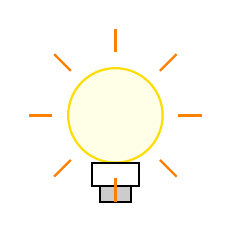
\begin{tikzpicture}[scale=1.0] 
                \draw[yellow!80!orange, thick, fill=yellow!10] (0,0) circle (0.6);
                \draw[thick] (-0.3,-0.6) rectangle (0.3,-0.9);
                \draw[thick, fill=gray!40] (-0.2,-0.9) rectangle (0.2,-1.1);
                \foreach \a in {0,45,...,315} \draw[orange, thick] (\a:0.8) -- (\a:1.1);
            \end{tikzpicture}
        \end{column}
        \begin{column}{0.8\textwidth}
            The \textit{"MapReduce"} paper by Dean \& Ghemawat:
            \begin{itemize}
                \item \textbf{Abstraction:} Simplified distributed math into Map/Reduce.
                \item \textbf{Fault Tolerance:} Hardware failure is now a software problem.
                \item \textbf{Data Locality:} "Move the computation, not the data."
            \end{itemize}
        \end{column}
    \end{columns}
    
    \vfill
    \begin{alertblock}{The Catalyst for Innovation}
        By sharing this blueprint, Google allowed the community to build \textbf{Apache Hadoop}, moving beyond the "Single Giant" era.
    \end{alertblock}
\end{frame}

% --- Slide 3: Evolution of Speed (Hadoop vs Spark) ---
\begin{frame}{From the "Basement" to the "Desk"}
    \begin{columns}
        \begin{column}{0.75\textwidth}
            \begin{itemize}
                \item \textbf{Hadoop Era (2006):} Relied on Disk. Like a librarian walking to the \textbf{basement} for every book.
                \item \textbf{Spark Era (2014):} Uses RAM (RDDs). The librarian keeps everything on the \textbf{desk}.
            \end{itemize}
        \end{column}
        \begin{column}{0.25\textwidth}
            \centering
            % --- TikZ Level Up (Scaled 1.6x) ---
            
\begin{tikzpicture}[scale=0.65] 
                \draw[cyan, line width=4pt, ->] (0,0) -- (0,3);
                \node[cyan, font=\small\bfseries, align=center] at (0,3.6) {LEVEL\\UP};
            \end{tikzpicture}
        \end{column}
    \end{columns}

    \vfill
    \begin{table}
        \centering
        \footnotesize
        \begin{tabular}{|l|c|c|}
            \hline
            \textbf{Feature} & \textbf{Hadoop (Disk)} & \textbf{Spark (RAM)} \\ \hline
            Processing Speed & 1x & \textbf{100x Faster} \\ \hline
            Data Access & Sequential & \textbf{Instant (RDD)} \\ \hline
        \end{tabular}
    \end{table}
\end{frame}

% --- Slide 4: Spark Architecture \& The New Bottleneck ---
\begin{frame}{Spark Architecture \& The New Bottleneck}
    \begin{itemize}
        \item \textbf{The Setup:} Database partitioned across the cluster's RAM.
        \item \textbf{The Pattern:} Candidates ($C_k$) are broadcast to every worker.
    \end{itemize}

    \vfill
    \begin{alertblock}{The CPU Wall}
        Data is now in RAM, so the disk is no longer the problem. The new bottleneck is the \textbf{CPU} searching millions of candidates per second.
    \end{alertblock}

    \vfill
    \begin{center}
        \footnotesize \itshape Coming up: A deep dive into the \textbf{Data Structures} that will solve this bottleneck...
    \end{center}
\end{frame}

\section{Literature Overview}

% --- Slide 1: The FIM Landscape ---
\begin{frame}[t]{The Evolution of FIM Environments}
    \vspace{0.2cm}
    Before addressing the HTT, we must categorize how FIM has adapted to shifting hardware constraints:
    
    \vspace{0.4cm}
    \renewcommand{\arraystretch}{1.3}
    \centering
    \begin{tabularx}{\textwidth}{l l l >{\raggedright\arraybackslash}X}
        \rowcolor{SecondaryColor!20}
        \textbf{Era} & \textbf{Algorithm} & \textbf{Storage} & \textbf{Main Bottleneck} \\ \hline
        Classic & Apriori & Local RAM & Memory Capacity \\
        Distributed & PFP (Hadoop) & HDFS (Disk) & \textbf{Network \& Disk I/O} \\
        \textbf{Modern} & \textbf{Spark} & \textbf{RDD (RAM)} & \textbf{CPU (Search)} \\ \hline
    \end{tabularx}

    \vspace{0.6cm}
    \begin{itemize}
        \item \textbf{The Shift:} Spark's RDD persistence effectively "solved" the I/O problem.
        \item \textbf{The New Reality:} When data is already in RAM, the time spent traversing pointer-heavy structures becomes the dominant cost.
    \end{itemize}
\end{frame}

% --- Slide 2: The Migration from MapReduce to Spark ---
\begin{frame}[t]{Architectural Migration: Hadoop to Spark}
    \begin{itemize}
        \item \textbf{Hadoop Era (PFP, PARMA, FPC/DPC):}
        \begin{itemize}
            \item \small MapReduce algorithms faced high latency due to launching new jobs for every iteration.
            \item \small \textbf{Costly I/O:} Constant disk read/write operations for intermediate results.
        \end{itemize}
        \item \textbf{The Spark Era (YAFIM, R-Apriori):}
        \begin{itemize}
            \item \small \textbf{YAFIM:} The pioneer Spark-based Apriori. It eliminated disk I/O, proving that in-memory RDD computation is 25x faster.
        \end{itemize}
    \end{itemize}

    \begin{center}
        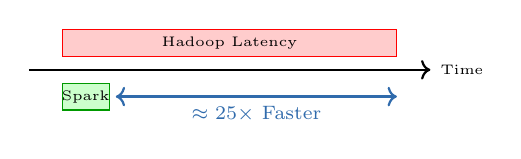
\begin{tikzpicture}[scale=0.85]
            % X-Axis
            \draw[thick, ->] (0,0) -- (6,0) node[right, font=\tiny] {Time};
            % Hadoop Bar
            \draw[fill=red!20, draw=red] (0.5,0.2) rectangle (5.5,0.6) node[pos=.5, font=\tiny] {Hadoop Latency};
            % Spark Bar
            \draw[fill=green!20, draw=green!60!black] (0.5,-0.6) rectangle (1.2,-0.2) node[pos=.5, font=\tiny] {Spark};
            % Speedup Annotation
            \draw[<->, thick, SecondaryColor] (1.3,-0.4) -- (5.5,-0.4);
            \node[font=\scriptsize, SecondaryColor, below] at (3.4,-0.4) {$\approx 25\times$ Faster};
        \end{tikzpicture}
    \end{center}

    \begin{alertblock}{Transition Summary}
        \footnotesize Shift from \textbf{Disk Latency} to \textbf{In-Memory Search Speed}.
    \end{alertblock}
\end{frame}

% --- Slide 3: Pruning Strategy ---
\begin{frame}[t]{Pruning Strategies}
    \begin{itemize}
        \item \textbf{The Goal:} Reduce the number of candidate itemsets that need to be counted.
        \item \textbf{The Logic:}
        \begin{itemize}
            \item \small If an itemset is identified as non-frequent through pruning, it is discarded instantly.
            \item \small Only the remaining "potential" candidates proceed to the actual counting phase.
        \end{itemize}
    \end{itemize}

    \begin{center}
        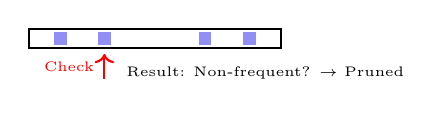
\begin{tikzpicture}[scale=0.8]
            \draw[thick] (0,0) rectangle (4,0.3);
            \foreach \x in {0.5,1.2,2.8,3.5} \fill[AlertColor] (\x-0.1,0.05) rectangle (\x+0.1,0.25);
            \draw[->, thick, red] (1.2,-0.5) -- (1.2,-0.1) node[midway, left, font=\tiny] {Check};
            \node[font=\tiny, right] at (1.4,-0.4) {Result: Non-frequent? $\to$ Pruned};
        \end{tikzpicture}
    \end{center}
    
    \begin{alertblock}{Focus}
        \footnotesize Pruning effectively reduces the total \textbf{candidate count} before the search begins.
    \end{alertblock}
\end{frame}

% --- Slide 4: Data Structure Innovations (Balanced Height Version) ---
\begin{frame}[t]{Data Structures in Related Work}
    Beyond global pruning, researchers explored local memory-mapping:
    
    \begin{itemize}
        \item \small \textbf{Boolean Vectors (DFIMA):} Uses bitwise matrix pruning to handle candidates efficiently within Spark.
        \item \small \textbf{Array Vectors (Yang et al.):} Maps the database into contiguous memory for fast parallel iteration.
        \item \small \textbf{Ultrametric Trees (FiDoop):} Uses the \textit{FIU-Tree} to provide a more compressed representation.
    \end{itemize}

    \vspace{0.1cm}
    \begin{columns}[T]
        \begin{column}{0.48\textwidth}
            \begin{alertblock}{Pointer-Based (Legacy)}
                \scriptsize \centering
                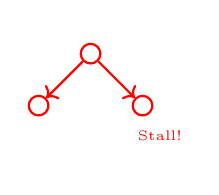
\begin{tikzpicture}[scale=1.1]
                    \tikzset{every node/.style={draw, circle, inner sep=2.5pt}}
                    \tikzset{every path/.style={->,red,thick}}
                    
                    \node (a) at (0,0.6) {};
                    \node (b) at (-0.6,0.0) {};
                    \node (c) at (0.6,0.0) {};
                    
                    \draw (a) -- (b); 
                    \draw (a) -- (c);
                    
                    \node[draw=none, circle=none, red, font=\tiny] at (0.8,-0.35) {Stall!};

                    \path (0,0.5) -- (0,0.9); 
                \end{tikzpicture}\\
                Memory Fragmentation
            \end{alertblock}
        \end{column}
        
        \begin{column}{0.48\textwidth}
            \begin{alertblock}{Direct Access (Proposed)}
                \scriptsize \centering
                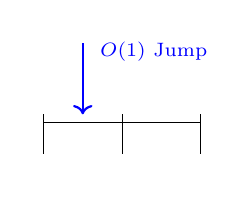
\begin{tikzpicture}[scale=1.0]
                    \draw (0,-0.4) grid (2,0.1);
                    \draw[->,blue,thick] (0.5,1.0) -- (0.5,0.1);
                    \node[blue, font=\scriptsize] at (1.4,0.9) {$O(1)$ Jump};
                    
                    \path[use as bounding box] (-0.2,-0.6) rectangle (2.2,1.2);
                \end{tikzpicture}\\
                Cache-Friendly
            \end{alertblock}
        \end{column}
    \end{columns}
\end{frame}

% --- Slide 5: The Remaining Challenge ---
\begin{frame}[t]{The Remaining Challenge}
    \begin{itemize}
        \item \textbf{The Progress:} Systems have moved from slow Disk I/O (Hadoop) to fast In-Memory RDDs (Spark).
        \item \textbf{The Success:} Modern techniques already use \textbf{Pruning} to reduce the number of candidates.
        \item \textbf{The Problem:} Even with fewer candidates, searching for itemsets inside an RDD partition is still the bottleneck.
    \end{itemize}

    \vspace{1.0cm}
    \begin{alertblock}{The Main Question}
        \centering
        \large \textit{"If the data is already in RAM, why is the search inside the partition still the bottleneck?"}
    \end{alertblock}
\end{frame}

% sections/06_data_structures.tex

\section{Proposed Data Structures}

% --- Slide: HT Architecture ---
\begin{frame}[t]{The Hash Tree (HT): Internal Architecture}
    \begin{columns}
        \begin{column}{0.5\textwidth}
            \begin{itemize}
                \item \textbf{Routing Logic:} Internal nodes use a hash function $h(i)$ to select the branch.
                \item \textbf{Leaf Buckets:} Fixed-size containers for candidate verification.
            \end{itemize}
        \end{column}
        \begin{column}{0.5\textwidth}
            \centering
            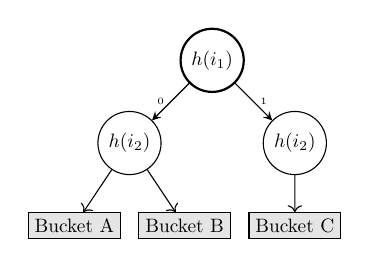
\begin{tikzpicture}[scale=0.7, every node/.style={scale=0.7}]
                \node[draw, circle, thick] (R) at (2,3) {$h(i_1)$};
                \node[draw, circle] (C1) at (0.5,1.5) {$h(i_2)$};
                \node[draw, circle] (C2) at (3.5,1.5) {$h(i_2)$};
                \node[draw, rectangle, fill=gray!20] (L1) at (-0.5,0) {Bucket A};
                \node[draw, rectangle, fill=gray!20] (L2) at (1.5,0) {Bucket B};
                \node[draw, rectangle, fill=gray!20] (L3) at (3.5,0) {Bucket C};
                
                \draw[->, >=stealth] (R) -- (C1) node[midway, left] {\tiny 0};
                \draw[->, >=stealth] (R) -- (C2) node[midway, right] {\tiny 1};
                \draw[->] (C1) -- (L1);
                \draw[->] (C1) -- (L2);
                \draw[->] (C2) -- (L3);
            \end{tikzpicture}
        \end{column}
    \end{columns}
    \vfill
    \begin{alertblock}{Design Intent}
        To verify $\{1, 5\}$, the system calculates $h(1)$ then $h(5)$ to reach a specific bucket. This minimizes memory footprint but increases computational cost.
    \end{alertblock}
\end{frame}

% --- Slide: HT Bottlenecks ---
\begin{frame}[t]{The Hash Tree (HT): Performance Bottlenecks}
    \begin{alertblock}{The "Bucket Overflow" Phenomenon}
        When $h(i)$ produces collisions, the leaf bucket becomes a long linked list.
    \end{alertblock}

    \begin{itemize}
        \item \textbf{Search Breakdown:} Verification degrades from a "smart jump" to a \textbf{linear scan} ($O(n)$).
        \item \textbf{The Spark Tax:} On Spark RDDs, the constant calculation of $h(i)$ for millions of records creates a bottleneck that prevents high-throughput scaling.
    \end{itemize}
    
    \vfill
    \centering
    \begin{tikzpicture}[scale=0.9]
        \node[draw, rectangle, minimum width=3.5cm, fill=red!10, thick] (B) {Bucket Overflow};
        \node[draw, rectangle, right=0.5cm of B, font=\tiny] (i1) {$\{a,b,c\}$};
        \node[draw, rectangle, right=0cm of i1, font=\tiny] (i2) {$\{a,d,e\}$};
        \node[draw, rectangle, right=0cm of i2, font=\tiny] (i3) {$\{b,c,e\}$};
        \node[draw, rectangle, right=0cm of i3, font=\tiny] (i4) {\dots};
        \draw[thick, red, ->] (B.east) -- (i1.west);
    \end{tikzpicture}
\end{frame}

% --- Slide: The Trie ---
\begin{frame}[t]{The Trie (Prefix Tree): Structural Optimization}
    \begin{columns}
        \begin{column}{0.4\textwidth}
            \textbf{Prefix Sharing:}
            \begin{itemize}
                \item Itemsets: $\{a,b,c\}$ and $\{a,b,d\}$.
                \item $\{a,b\}$ is stored once, exploiting commonality.
            \end{itemize}
        \end{column}
        \begin{column}{0.6\textwidth}
            \centering
            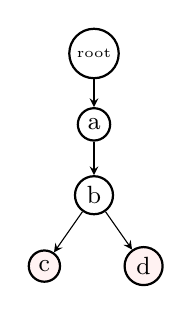
\begin{tikzpicture}[
                node/.style={draw, circle, inner sep=2pt, font=\small, thick},
                edge/.style={->, >=stealth},
                scale=0.9
            ]
                \node[node] (R) at (0,0) {\tiny root};
                \node[node] (A) at (0,-1) {a};
                \node[node] (B) at (0,-2) {b};
                \node[node, fill=red!5] (C) at (-0.7,-3) {c};
                \node[node, fill=red!5] (D) at (0.7,-3) {d};
                
                \draw[edge] (R) -- (A);
                \draw[edge] (A) -- (B);
                \draw[edge] (B) -- (C);
                \draw[edge] (B) -- (D);
            \end{tikzpicture}
        \end{column}
    \end{columns}
    \vfill
    \begin{alertblock}{The Sibling Problem}
        Finding 'd' after 'b' requires searching through all of 'b's children. In large datasets, this search is $O(\log k)$ or $O(k)$ depending on the node implementation.
    \end{alertblock}
\end{frame}

% --- Slide: The HTT Solution ---
\begin{frame}[t]{The Hash Table Trie (HTT) Hybrid}
    \vspace{-0.2cm}
    \textbf{The Innovation: Localized Map Lookup}
    
    \begin{center}
    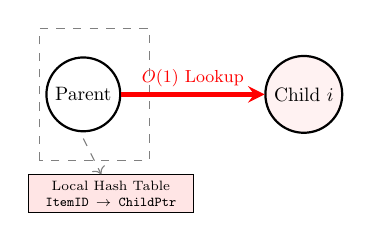
\begin{tikzpicture}[scale=0.7, every node/.style={transform shape}]
        \node[draw, circle, thick] (P) at (0,0) {Parent};
        \node[draw, circle, thick, fill=red!5] (C) at (4,0) {Child $i$};
        
        \draw[dashed, gray] (-0.8,-1.2) rectangle (1.2,1.2);
        \node[draw, rectangle, fill=red!10, minimum width=3cm, align=center, font=\scriptsize] (HT) at (0.5,-1.8) {Local Hash Table\\ \texttt{ItemID $\rightarrow$ ChildPtr}};
        
        \draw[->, ultra thick, red, >=stealth] (P) -- (C) node[midway, above] {\small $O(1)$ Lookup};
        \draw[->, thin, gray, dashed] (0,-0.8) -- (HT);
    \end{tikzpicture}
    \end{center}

    \vspace{-0.4cm}

    \begin{table}[]
        \centering
        \scriptsize
        \begin{tabular}{l|c|c|c}
            \toprule
            \textbf{Metric} & \textbf{HT} & \textbf{Standard Trie} & \textbf{HTT (Proposed)} \\ \midrule
            Sibling Lookup & $O(n)$ scan & $O(\log k)$ search & $\mathbf{O(1)}$ \textbf{lookup} \\ 
            Traversal Time & $O(k \cdot h)$ & $O(L \cdot \log k)$ & $\mathbf{O(L)}$ \\ 
            Spark Reality & CPU Bound & Memory Latency & \textbf{Max Throughput} \\ \bottomrule
        \end{tabular}
    \end{table}

    \vspace{-0.2cm}

    \begin{alertblock}{Technical Verdict}
        By embedding hash tables \textit{inside} the Trie nodes, the \textbf{HTT} eliminates the branching factor ($k$) from the complexity, maximizing Spark's RDD throughput.
    \end{alertblock}
\end{frame}

% sections/07_results.tex

\section{Experimental Results}

% --- Slide 1: Hardware Specs ---
\begin{frame}{Experimental Results: Hardware Specifications}
  \begin{columns}[onlytextwidth, T]
    \column{0.6\textwidth}
      \begin{itemize}
        \item \textbf{PC Build (Workstation):} 
        \begin{itemize}
          \item \textbf{CPU:} Intel Xenon CPU E5-2620@2.10 GHz with 24 cores \textit{(Inferred Dual-Processor setup)}.
          \item \textbf{RAM:} 16 GB DDR3 \textit{(Inferred Quad-Channel configuration)}.
          \item \textbf{Storage:} 1 TB of disk storage \textit{(Inferred HDD for HDFS layer)}.
        \end{itemize}
      \end{itemize}

    \column{0.4\textwidth}
      \centering
      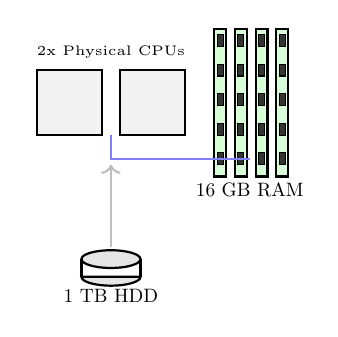
\begin{tikzpicture}[scale=0.75]
        \draw[thick, fill=gray!10] (0,1.2) rectangle (1.1,2.3);
        \draw[thick, fill=gray!10] (1.4,1.2) rectangle (2.5,2.3);
        \node at (1.25,2.6) {\tiny 2x Physical CPUs};

        \foreach \x in {0, 0.35, 0.7, 1.05} {
          \draw[thick, fill=green!15] (3.0+\x, 0.5) rectangle (3.0+\x+0.2, 3);
          \foreach \y in {0.7, 1.2, 1.7, 2.2, 2.7}
            \draw[fill=black!80] (3.0+\x+0.05, \y) rectangle (3.0+\x+0.15, \y+0.2);
        }
        \node[below, scale=0.7] at (3.6,0.5) {16 GB RAM};
        
        \begin{scope}[yshift=-1.2cm, xshift=1.25cm]
            \draw[thick, fill=gray!20] (0,0.3) ellipse (0.5 and 0.15);
            \draw[thick] (-0.5,0) -- (-0.5,0.3);
            \draw[thick] (0.5,0) -- (0.5,0.3);
            \draw[thick, fill=gray!20] (-0.5,0) arc (180:360:0.5 and 0.15) -- (0.5,0) -- cycle;
            \node[below, scale=0.7] at (0,-0.1) {1 TB HDD};
        \end{scope}
        
        \draw[thick, blue!50] (1.25,1.2) -- (1.25,0.8) -- (3.6,0.8);
        \draw[thick, gray!50, ->] (1.25,-0.7) -- (1.25,0.7);
      \end{tikzpicture}
  \end{columns}

  \vfill
  \begin{alertblock}{Hardware Capacity}
    The dual-processor setup provides 24 execution threads, while the quad-channel memory configuration ensures high data transfer speeds between the RAM and the CPUs.
  \end{alertblock}
\end{frame}

% --- Slide 2: Software Stack ---
\begin{frame}{Experimental Results: Software \& Memory Mode}
  \begin{columns}[onlytextwidth, T]
    \column{0.6\textwidth}
      \begin{itemize}
        \item \textbf{Software Stack:} 
        \begin{itemize}
          \item \textbf{OS:} Ubuntu 14.04 (64-bit).
          \item \textbf{Frameworks:} Spark 2.1.1, Hadoop 2.6.0.
          \item \textbf{Language:} Java 7 / Scala 2.11.8.
        \end{itemize}
        \vfill
        \item \textbf{Memory Mode:} 
        \begin{itemize}
          \item \textbf{Level:} \texttt{MEMORY\_ONLY}.
          \item \textbf{Strategy:} RDDs are cached in RAM.
          \item \textbf{Impact:} Bypasses Disk I/O bottlenecks during $L_k$ generation.
        \end{itemize}
      \end{itemize}

    \column{0.4\textwidth}
      \centering
      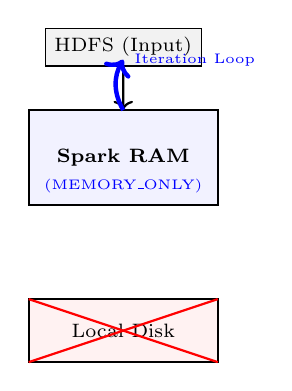
\begin{tikzpicture}[scale=0.8]
        \node[draw, fill=gray!10] (hdfs) at (1.5,4) {\scriptsize HDFS (Input)};
        \draw[thick, fill=blue!5] (0,1.5) rectangle (3,3);
        \node at (1.5,2.25) {\scriptsize \textbf{Spark RAM}};
        \node[blue] at (1.5,1.8) {\tiny (MEMORY\_ONLY)};
        \draw[thick, fill=red!5] (0,0) rectangle (3,-1);
        \node at (1.5,-0.5) {\scriptsize Local Disk};
        \draw[red, thick] (0,0) -- (3,-1); \draw[red, thick] (3,0) -- (0,-1);
        \draw[->, thick] (hdfs) -- (1.5,3);
        \draw[->, blue, ultra thick] (1.5,3) to [bend left] (1.5,3.8) node[right] {\tiny Iteration Loop};
      \end{tikzpicture}
  \end{columns}
\end{frame}

% --- Slide 3: Performance I (2x2 Plot - Mushroom/Chess) ---
\begin{frame}{Performance Analysis: Datasets (a) to (d)}
    \vspace{-0.2cm}
    \begin{center}
        
\includegraphics[height=0.72\textheight, width=0.95\textwidth, keepaspectratio]{plots_2x2.png}
    \end{center}
    \vspace{-0.3cm}
    \begin{itemize}
        \item \footnotesize \textbf{Observation:} On dense datasets like \textit{Mushroom} and \textit{Chess}, HTT maintains a steady \textbf{2x speedup} by optimizing CPU cache usage during RDD lookups.
    \end{itemize}
\end{frame}

% --- Slide 4: Performance II (Triangular Plot - BMS) ---
\begin{frame}{Performance Analysis: Datasets (e) to (g)}
    \vspace{-0.2cm}
    \begin{center}
        
\includegraphics[height=0.72\textheight, width=0.95\textwidth, keepaspectratio]{plots_triangular.png}
    \end{center}
    \vspace{-0.3cm}
    \begin{itemize}
        \item \footnotesize \textbf{Observation:} For sparse datasets (BMS1/BMS2), the efficiency of the Trie-based architecture becomes even more apparent, achieving an \textbf{8x performance gain}.
    \end{itemize}
\end{frame}

% --- Slide 5: Summary Table ---
\begin{frame}{Experimental Results: Summary Table}
    \centering
    \begin{beamercolorbox}[sep=6pt,center,rounded=true]{block body}
        \textbf{Relative Speedup vs. Hash Tree (HT)}
    \end{beamercolorbox}
    \vspace{0.1cm}
    \begin{tabular}{|l|c|c|c|}
        \hline
        \textbf{Dataset} & \textbf{HT (Baseline)} & \textbf{Trie} & \textbf{HTT} \\ \hline
        BMS1 / BMS2      & 1.0x                & \textbf{> 8.0x} & \textbf{> 8.0x} \\ \hline
        T40I10D100K      & 1.0x                & 5.8x            & \textbf{6.1x}   \\ \hline
        Mushroom / Chess & 1.0x                & 1.9x            & \textbf{2.1x}   \\ \hline
    \end{tabular}
    \vfill
    \begin{alertblock}{The RDD Conclusion}
        \small The results validate that within Spark, the computational efficiency of $O(1)$ lookups in the Hash Table Trie (HTT) justifies its memory footprint.
    \end{alertblock}
\end{frame}

% sections/08_conclusion.tex

\section{Conclusion}
\begin{frame}{Conclusion: The Sequential Context}
    \begin{itemize}
        \item \textbf{Theoretical Expectation:} 
        \begin{itemize}
            \item The \textbf{Hash Table Trie} was designed to accelerate itemset traversal by combining Trie logic with hashing.
        \end{itemize}
        \vfill
        \item \textbf{Previous Practical Failure:} 
        \begin{itemize}
            \item In earlier sequential implementations, where \textbf{memory was a strict bottleneck}, the hashing overhead caused it to underperform.
            \item It was often documented as the least efficient variant in non-distributed settings.
        \end{itemize}
    \end{itemize}
\end{frame}

\begin{frame}{Conclusion: The Spark Paradigm Shift}
    \begin{itemize}
        \item \textbf{Distributed Advantage:} 
        \begin{itemize}
            \item Within Spark's \textbf{distributed memory (RDD)} architecture, the Hash Table Trie finally realizes its theoretical efficiency.
        \end{itemize}
        \vfill
        \item \textbf{Benchmark Results:} 
        \begin{itemize}
            \item Experimental data shows it performs \textbf{significantly better} than the traditional Hash Tree.
            \item It maintains a slight edge over the standard Trie across most datasets.
        \end{itemize}
    \end{itemize}
\end{frame}

\begin{frame}{Conclusion: Final Verdict}
    \begin{itemize}
        \item \textbf{In-Memory Optimization:} 
        \begin{itemize}
            \item Memory-optimized structures are the key to high-performance FIM on Spark.
        \end{itemize}
        \vfill
        \item \textbf{Summary:}
        \begin{itemize}
            \item The \textbf{Hash Table Trie}, once considered the ``worst'' in sequential settings, is now the most robust choice for RDD-based Apriori.
            \item Infrastructure alone (Spark) isn't enough; the underlying \textbf{data structure} must evolve to match the hardware.
        \end{itemize}
    \end{itemize}
\end{frame}

% sections/09_references.tex

\section{References}
\begin{frame}{References}
    \footnotesize
    \begin{thebibliography}{99}
        \bibitem{Singh2019}
        P. Singh, S. Singh, P. K. Mishra, and R. Garg.
        \newblock \textbf{A data structure perspective to the RDD-based Apriori algorithm on Spark.}
        \newblock \textit{Int. J. Inf. Technol.}, 14(3):1585--1594, 2019.
        
        \vspace{0.4cm}
        
        \bibitem{Zaki2000}
        M. J. Zaki.
        \newblock \textbf{Scalable algorithms for association mining.}
        \newblock \textit{IEEE Trans. Knowl. Data Eng.}, 12(3):372--390, 2000.
        
        \vspace{0.4cm}
        
        \bibitem{Agrawal1994}
        R. Agrawal and R. Srikant.
        \newblock \textbf{Fast algorithms for mining association rules.}
        \newblock \textit{Proc. 20th Int. Conf. Very Large Data Bases (VLDB)}, 487--499, 1994.
    \end{thebibliography}
\end{frame}

% sections/10_qa.tex

\begin{frame}[plain]
  \centering
  \vfill
  \begin{beamercolorbox}[sep=12pt,center,rounded=true,shadow=true]{palette primary}
    \usebeamerfont{title}\Huge Questions? \\
    \vspace{0.3cm}
    \usebeamerfont{title}\Large Obrigado! \raisebox{-1pt}{\(\mathbf{\ddot{\smile}}\)}
  \end{beamercolorbox}
  \vfill
  
  \begin{columns}[onlytextwidth, T]
    \column{0.5\textwidth}
      \centering
      \small \textbf{Distributed Work} \\
      \vspace{0.2cm}
      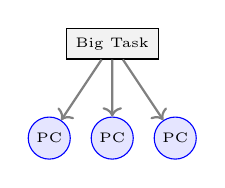
\begin{tikzpicture}[scale=0.8]
        % Top task
        \node[draw, fill=gray!10] (task) at (1,1.5) {\tiny Big Task};
        
        % Three small PC nodes
        \node[circle, draw=blue, fill=blue!10, inner sep=2pt] (p1) at (0,0) {\tiny PC};
        \node[circle, draw=blue, fill=blue!10, inner sep=2pt] (p2) at (1,0) {\tiny PC};
        \node[circle, draw=blue, fill=blue!10, inner sep=2pt] (p3) at (2,0) {\tiny PC};
        
        % Arrows showing the split
        \draw[->, thick, gray] (task) -- (p1);
        \draw[->, thick, gray] (task) -- (p2);
        \draw[->, thick, gray] (task) -- (p3);
      \end{tikzpicture}
      
    \column{0.5\textwidth}
      \centering
      \small \textbf{Speed Comparison} \\
      \vspace{0.2cm}
      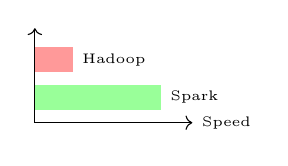
\begin{tikzpicture}[scale=0.8]
        % Simple Bar Chart
        \draw[->] (0,0) -- (2.5,0) node[right] {\tiny Speed};
        \draw[->] (0,0) -- (0,1.5);
        
        % Hadoop Bar (Short)
        \fill[red!40] (0,0.8) rectangle (0.6,1.2);
        \node[right] at (0.6,1.0) {\tiny Hadoop};
        
        % Spark Bar (Long)
        \fill[green!40] (0,0.2) rectangle (2.0,0.6);
        \node[right] at (2.0,0.4) {\tiny Spark};
      \end{tikzpicture}
  \end{columns}

  \vfill
  \textbf{\MyAuthor} \\
  \small \MyInstitute \\
  \vspace{0.2cm}
  \small \texttt{\MyEmail}
  \vfill
\end{frame}


\end{document}
